\section{Architecture and design}
\label{sec:architecture}

\subsection{Technical stack}

The stack was imposed by the subject: Python 3.13, FastAPI for the web service, Streamlit for
the interface and PostgreSQL for the database, developed on SSP Cloud. The dependencies of the
backend and of the frontend are managed separately with \texttt{uv}, and their exact versions are
locked in \texttt{uv.lock}, so that every member installs the same environment.

\subsection{Layered architecture}

The backend follows the layered architecture defined in the analysis report. Each layer only
calls the layer just below it.

\begin{table}[H]
\centering
\small
\begin{tabularx}{\textwidth}{l l X}
\toprule
\textbf{Layer} & \textbf{Folder} & \textbf{Role} \\
\midrule
Controller & \texttt{controller/} & HTTP endpoints (FastAPI routers): input validation, authentication, conversion of the errors into HTTP status codes \\
Schema & \texttt{schema/} & Pydantic models of the requests and responses \\
Service & \texttt{service/} & Business rules and computations, calls to the NASA API \\
DAO & \texttt{dao/} & SQL queries, one class per table or per feature \\
Business object & \texttt{business\_object/} & Domain classes: \texttt{Neo}, \texttt{Approach}, \texttt{User}, \texttt{Alert}, \texttt{Import}\dots \\
Utils & \texttt{utils/} & Security (passwords, JWT), logs, singleton, database reset \\
\bottomrule
\end{tabularx}
\caption{Layers of the backend}
\end{table}

The Streamlit frontend never reaches the database: every page calls the API through a single
HTTP client (\texttt{utils/api\_client.py}) which adds the authentication token to each request.
Figure~\ref{fig:packages} shows the packages and figure~\ref{fig:sequence} the path of a request
through the layers.

\begin{figure}[H]
  \centering
  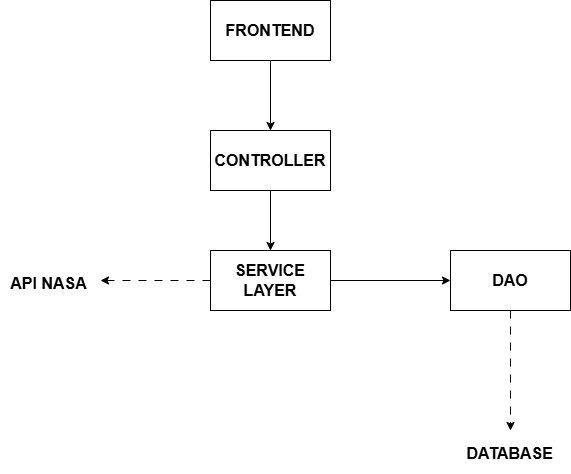
\includegraphics[width=0.75\textwidth]{diagramme_packages.drawio.png}
  \caption{Package diagram}
  \label{fig:packages}
\end{figure}

\begin{figure}[H]
  \centering
  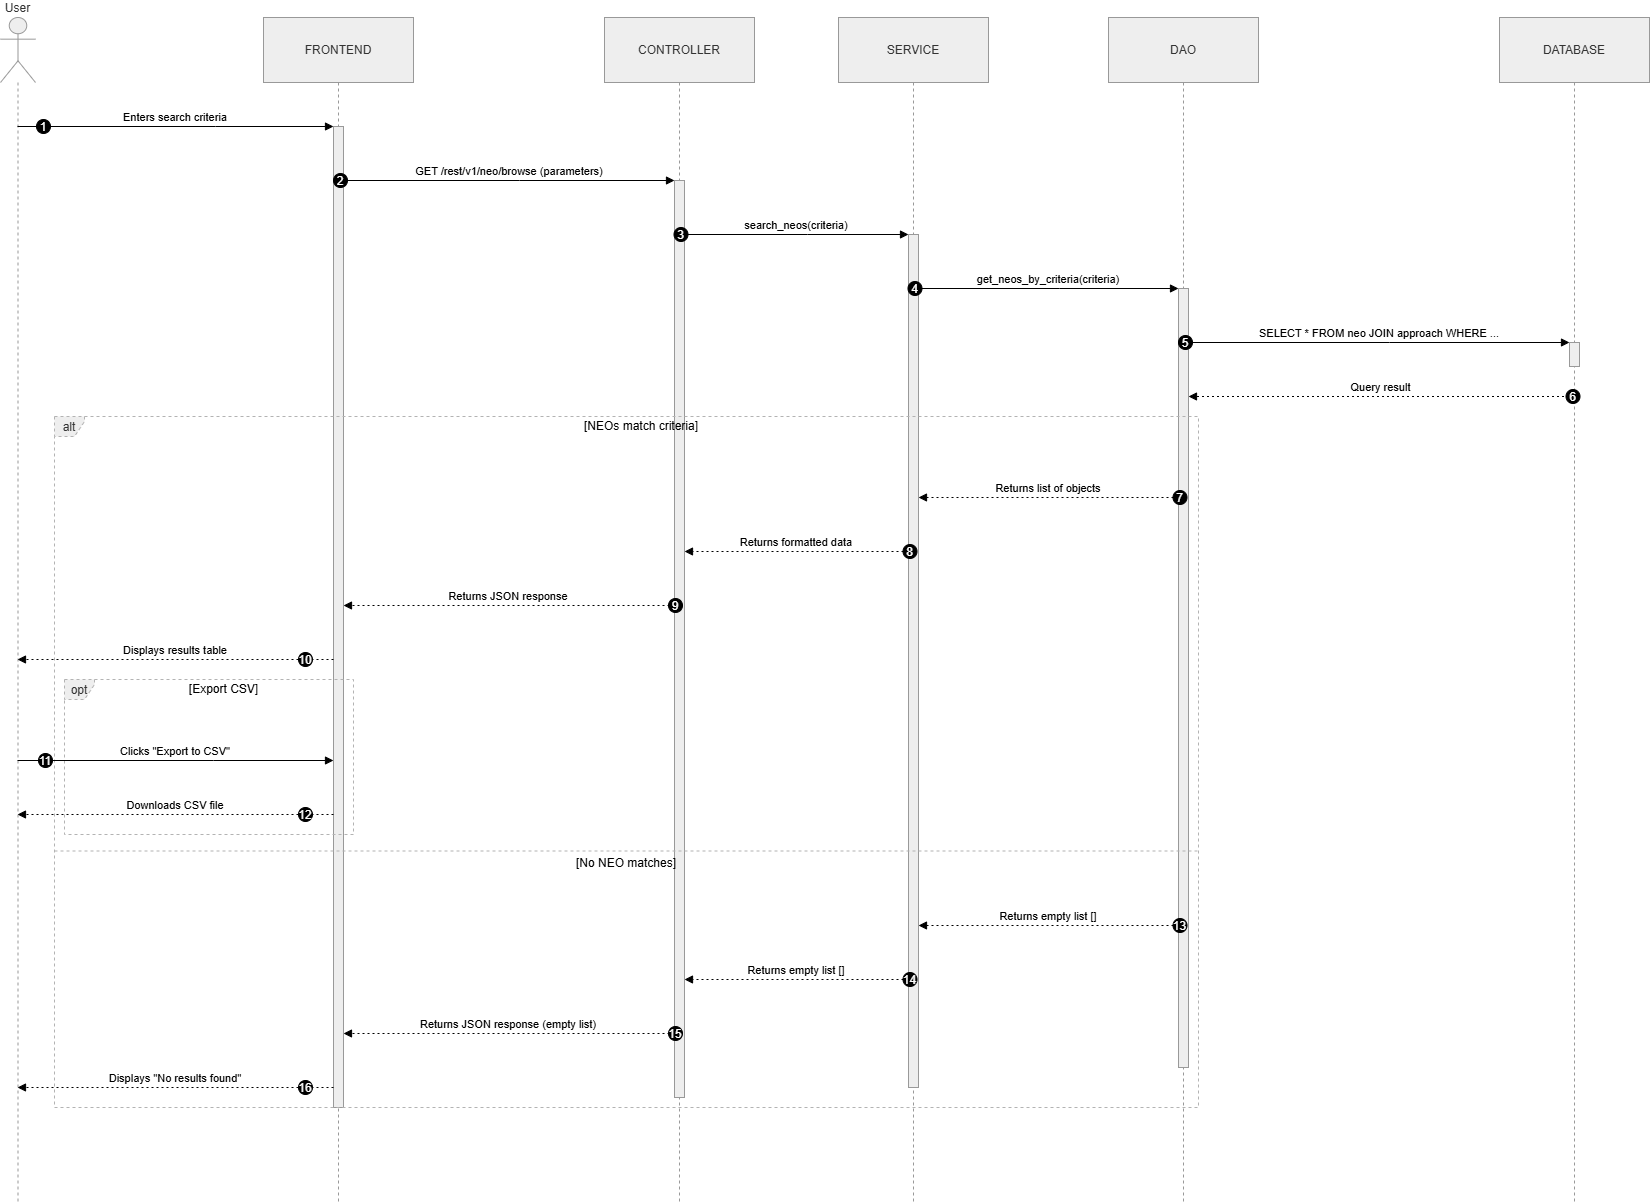
\includegraphics[width=0.75\textwidth]{diagramme_sequence.drawio.png}
  \caption{Sequence diagram of a request}
  \label{fig:sequence}
\end{figure}

\subsection{Data model}

The physical data model of the analysis report was kept (figure~\ref{fig:pdm}). Its main points
are:

\begin{itemize}
  \item \texttt{neo} and \texttt{approach} are two tables: the physical characteristics of an
  object are stored once, and each of its close approaches is a row of \texttt{approach}. The
  constraint \texttt{UNIQUE (neo\_id, approach\_day)} makes the imports idempotent: importing the
  same day twice updates the approach instead of duplicating it.
  \item \texttt{neo.nasa\_id} is unique but nullable: NEOs declared by users have no NASA
  identifier, and the import updates a NEO only through its \texttt{nasa\_id}
  (\texttt{ON CONFLICT (nasa\_id) DO UPDATE}), so it can never overwrite them.
  \item Diameters are stored in kilometres with six decimals (\texttt{NUMERIC(12, 6)}): with two
  decimals, every object smaller than 5~m was rounded to zero.
  \item The \texttt{import} table records each import with its period, its status and its
  counters. It is used to resume an interrupted import and to know when the next one is due.
\end{itemize}

\begin{figure}[H]
  \centering
  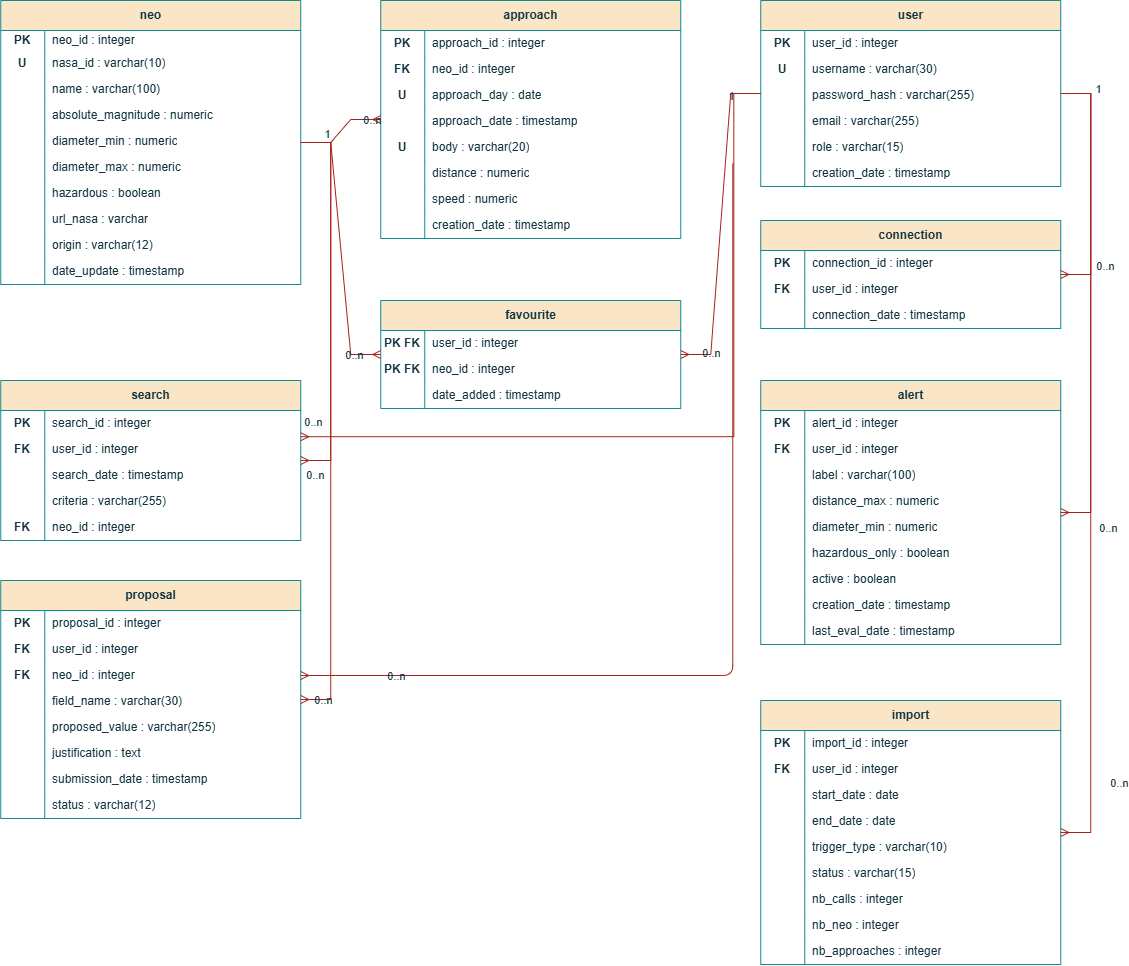
\includegraphics[width=0.75\textwidth]{databasediag.png}
  \caption{Physical data model}
  \label{fig:pdm}
\end{figure}

On its first start, the API creates the tables (\texttt{data/init\_db.sql}) and the seed data,
among which an administrator account (\texttt{data/pop\_db.sql}). On an existing database it only
applies a short list of schema fixes, so the data is kept.

\subsection{Main design choices}

\paragraph{Importing from the \texttt{/feed} endpoint.} As decided in the analysis, the data comes
from the NeoWs \texttt{/feed} endpoint, which returns all the approaches of a period of at most
seven days, rather than from \texttt{/neo/browse}, which returns objects one page at a time. The
import window is two years back and one year ahead: about 150 calls for the first import.

\paragraph{Imports in the background.} The first import lasts several minutes, much longer than
any HTTP timeout, and the free NASA key (\texttt{DEMO\_KEY}) only allows a few dozen calls per
hour. Imports therefore run in a background thread, one at a time. The window is cut into periods
of seven days; when the quota runs out in the middle, the import is recorded as \emph{partial},
with the last day that was saved, and the next import resumes from there.

\paragraph{One database connection per thread.} FastAPI runs the endpoints in a pool of threads,
and the import runs in its own thread. With a single shared \texttt{psycopg2} connection, all of
them shared the same transaction: one failing query aborted the requests running at the same
time. \texttt{DBConnection} is still a singleton, but it gives each thread its own connection.

\paragraph{Authentication.} The API uses JSON Web Tokens: an access token valid 30 minutes and a
refresh token valid 7 days. Every endpoint except login and registration requires an access
token; the user is read again from the database at each request, so a deleted account is
logged out at once. A user can only read and change their own favourites and alerts; the
administration endpoints require the \texttt{admin} role. Passwords are hashed with SHA-256,
salted with the username, and compared in constant time.
